%% LyX 1.4.3-5 created this file.  For more info, see http://www.lyx.org/.
%% Do not edit unless you really know what you are doing.
\documentclass[english]{beamer}
\usepackage[latin1]{inputenc}
\usepackage{amsmath}
\usepackage{graphicx}
\usepackage{amssymb}
\IfFileExists{url.sty}{\usepackage{url}}
                      {\newcommand{\url}{\texttt}}
\usepackage[authoryear]{natbib}

\makeatletter

%%%%%%%%%%%%%%%%%%%%%%%%%%%%%% LyX specific LaTeX commands.
%% A simple dot to overcome graphicx limitations
\newcommand{\lyxdot}{.}


%%%%%%%%%%%%%%%%%%%%%%%%%%%%%% Textclass specific LaTeX commands.
 \AtBeginDocument{
   \let\origtableofcontents=\tableofcontents
   \def\tableofcontents{\@ifnextchar[{\origtableofcontents}{\gobbletableofcontents}}
   \def\gobbletableofcontents#1{\origtableofcontents}
 }
 \makeatletter
 \long\def\lyxframe#1{\@lyxframe#1\@lyxframestop}%
 \def\@lyxframe{\@ifnextchar<{\@@lyxframe}{\@@lyxframe<*>}}%
 \def\@@lyxframe<#1>{\@ifnextchar[{\@@@lyxframe<#1>}{\@@@lyxframe<#1>[]}}
 \def\@@@lyxframe<#1>[{\@ifnextchar<{\@@@@@lyxframe<#1>[}{\@@@@lyxframe<#1>[<*>][}}
 \def\@@@@@lyxframe<#1>[#2]{\@ifnextchar[{\@@@@lyxframe<#1>[#2]}{\@@@@lyxframe<#1>[#2][]}}
 \long\def\@@@@lyxframe<#1>[#2][#3]#4\@lyxframestop#5\lyxframeend{%
   \frame<#1>[#2][#3]{\frametitle{#4}#5}}
 \makeatother
 \def\lyxframeend{} % In case there is a superfluous frame end
 \newenvironment{centercolumns}{\begin{columns}[c]}{\end{columns}}

%%%%%%%%%%%%%%%%%%%%%%%%%%%%%% User specified LaTeX commands.

\usepackage{listings}
\usetheme{Warsaw}
% or ...
%\usetheme{Antibes}	% tree outline, neat
%\usetheme{JuanLesPins}	% like Antibes, with shading
%\usetheme{Bergen}	% outline on side
%\usetheme{Luebeck}	% like Warsaw, square sides
%\usetheme{Berkeley}	% interesting left bar outline
%\usetheme{Madrid}	% clean, nice.  7/12 page numbers
%\usetheme{Berlin}	% dots show slide number
%\usetheme{Malmoe}	% OK, plain, unshaded
%\usetheme{Boadilla}	% nice, white bg, no top bar
%\usetheme{Marburg}	% nice, outline on right
%\usetheme{boxes}	% ???
%\usetheme{Montpellier}	% tree outline on top, plainish white
%\usetheme{Copenhagen}	% like Warsaw
%\usetheme{PaloAlto}	% looks good
%\usetheme{Darmstadt}	% like Warsaw with circle outline
%\usetheme{Pittsburgh}
%\usetheme{default}
%\usetheme{Rochester}	% like boxy, unshaded warsaw
%\usetheme{Dresden}	% circle outline on top
%\usetheme{Singapore}	% purple gradient top
%\usetheme{Frankfurt}	% like Warsaw with circle outline on top
%\usetheme{Szeged}
%\usetheme{Goettingen}	% light purple right bar outline
%\usetheme{Warsaw}
%\usetheme{Hannover}	% like Goett with bar on left
%\usetheme{compatibility}
%\usetheme{Ilmenau}

\setbeamercovered{transparent}
% or whatever (possibly just delete it)

%\usecolortheme{seahorse}
%\usecolortheme{rose}

% seems to fix typewriter font in outline header:
\usepackage{ae,aecompl}
\newcommand{\newblock}{}

\usepackage{babel}
\makeatother
\begin{document}

\title[The Gaussian Processes Latent Variable Model]{Hierarchical Gaussian Process Latent Variable Models}


\author[Neil Lawrence]{\textbf{Neil D. Lawrence} and Andrew J. Moore\\Machine Learning
Group\\School of Computer Science\\University of Manchester, U.K.}


\date{22nd June 2007}

\frame{\maketitle}


%\pgfdeclareimage[height=0.5cm]{sheffieldlogo}{../../../gp/tex/diagrams/sheffieldlogo.eps}

\logo{
\includegraphics[height=0.5cm]{../../../tex/inputs/sheffieldlogo}}

%\logo{\pgfuseimage{sheffieldlogo}}

% RPD:  can't get this to work on any template.  not present in Warsaw any way, it seems

% hmm, problem seems to be that it isn't copied to the tmp dir, probably becuase it doesn't have the

% filename extension (which is tacked on by pgf it seems)

%\AtBeginSubsection[]{

%  \frame<beamer>{ 

%    \frametitle{Outline}   

%    \tableofcontents[currentsection,currentsubsection] 

%  }

%}

%\beamerdefaultoverlayspecification{<+->}


\lyxframeend{}\lyxframe{Outline}

\tableofcontents{}


\lyxframeend{}


\lyxframeend{}\lyxframe{Online Resources}

\begin{block}
{All source code and slides are available online}
\begin{itemize}
\item This talk available from my home page (see talks link on left hand
side).
\item Examples shown are in the `oxford' toolbox (vrs 0.131).

\begin{itemize}
\item \url{http://www.cs.man.ac.uk/~neill/oxford/}.
\end{itemize}
\item And the `hgplvm' toolbox (vrs 0.1).

\begin{itemize}
\item \url{http://www.cs.man.ac.uk/~neill/hgplvm/}.
\end{itemize}
\item MATLAB commands used for examples given in \texttt{typewriter font}.
\end{itemize}
\end{block}

\lyxframeend{}\lyxframe{Curse of Dimensionality}

\begin{block}
{Incorporating assumptions about data structure}
\begin{itemize}
\item How do we model high dimensional data probabilistically?

\begin{enumerate}
\item Probabilistic models with sparse connectivity: tree structures, junction
trees, Markov random fields.

\begin{itemize}
\item Dictactes conditional independecies in the data.
\end{itemize}
\item Assume data inherently lives on a low dimensional manifold.

\begin{itemize}
\item Perhaps all data points are fully interdependent, but they live in
a low dimension space.
\end{itemize}
\end{enumerate}
\item Can we combine these two approaches in one model?
\end{itemize}
\end{block}

\lyxframeend{}\lyxframe{Modelling in High Dimensions}

\begin{block}
{Avoiding the Curse of Dimensionality}

%
\begin{figure}
\begin{centering}\only<1>{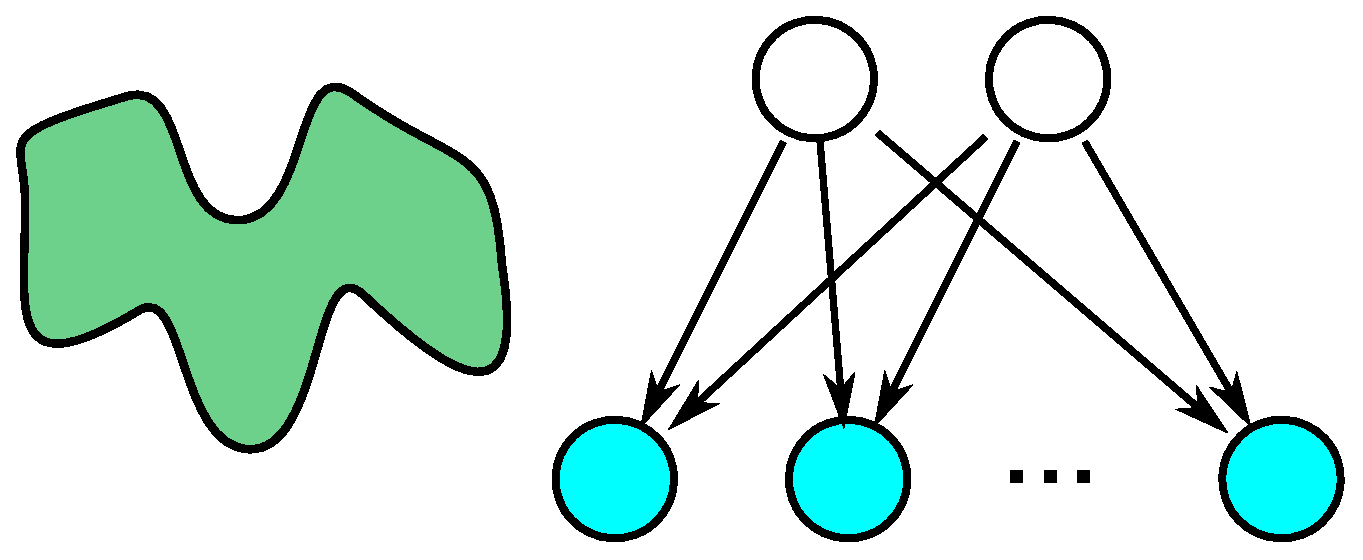
\includegraphics[width=0.8\textwidth]{\lyxdot \lyxdot /diagrams/nldrGraph}}\only<2>{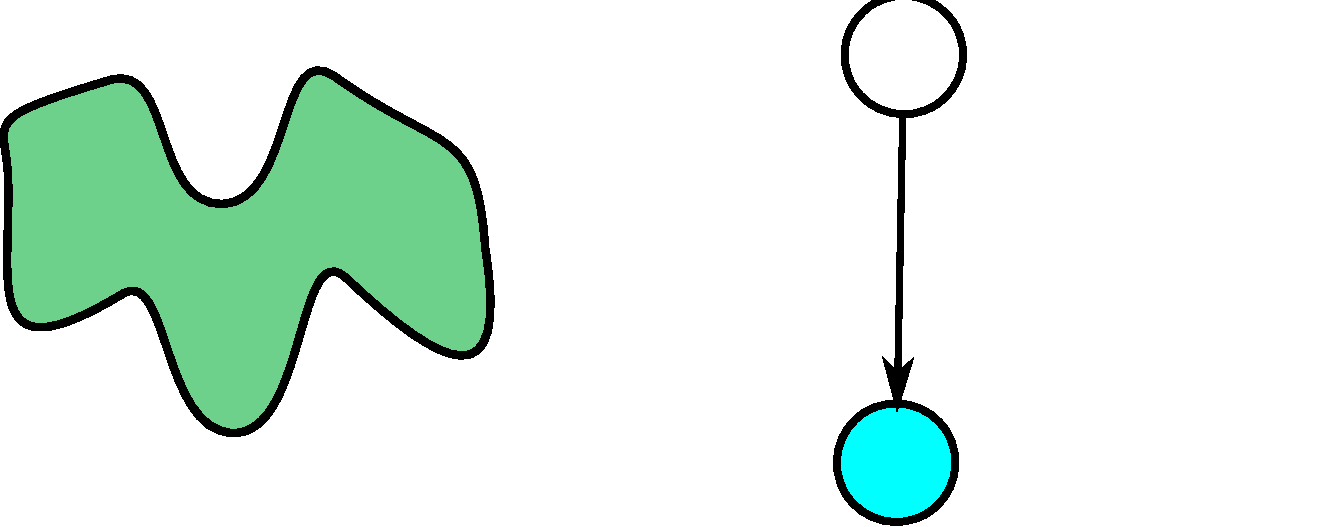
\includegraphics[width=0.8\textwidth]{\lyxdot \lyxdot /diagrams/nldrGraph2}}\only<3>{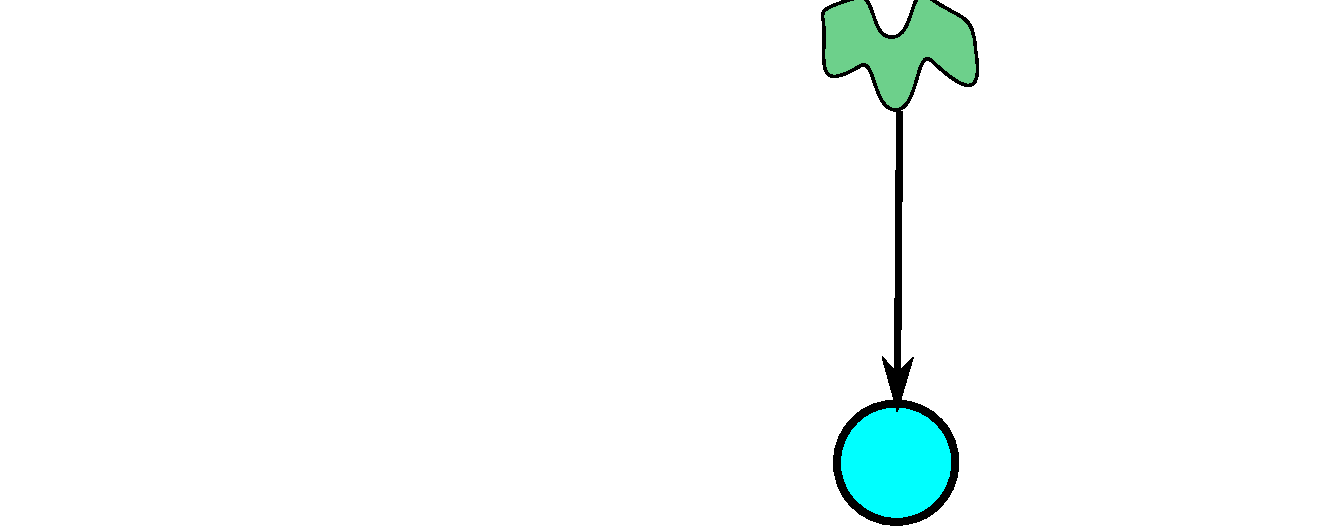
\includegraphics[width=0.8\textwidth]{\lyxdot \lyxdot /diagrams/nldrGraph3}}\only<4>{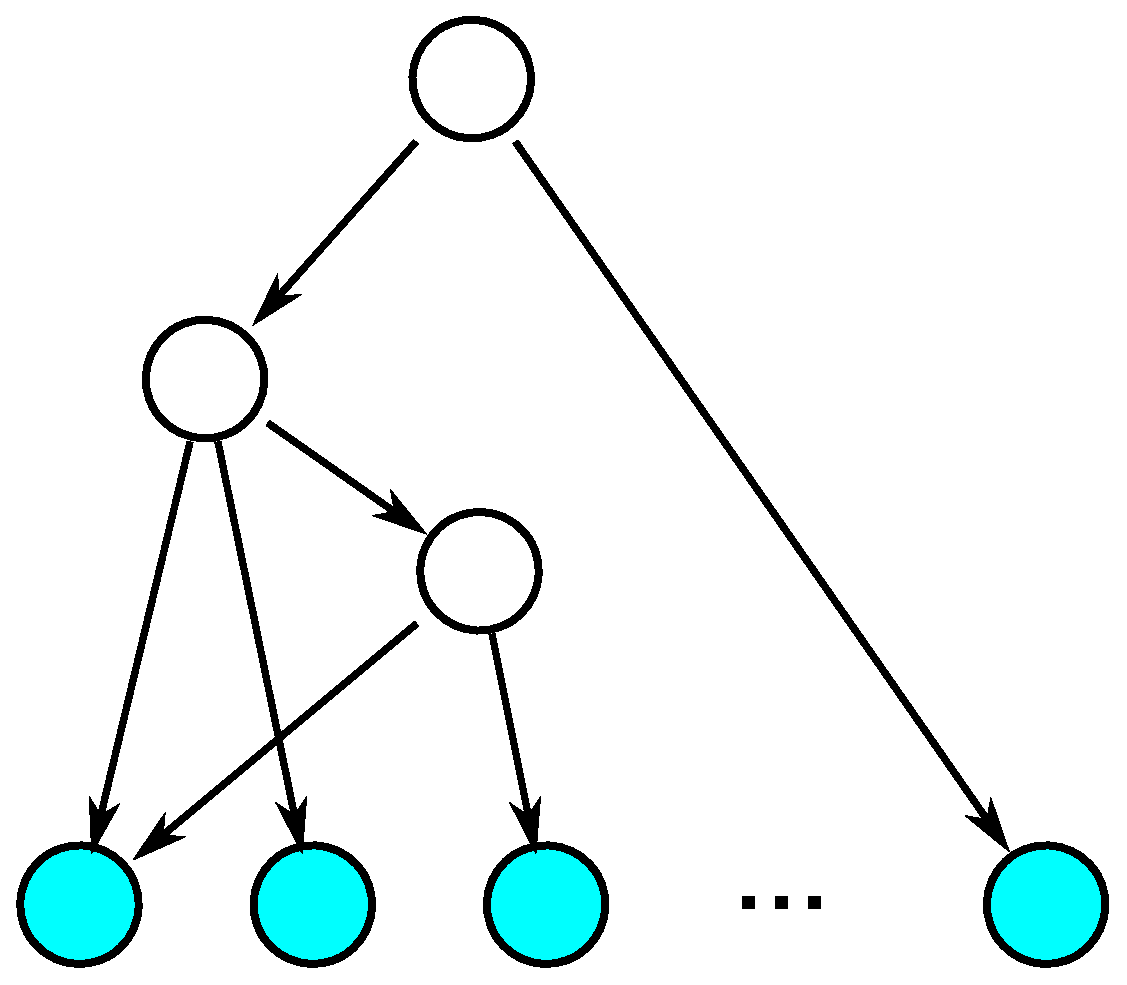
\includegraphics[width=0.5\textwidth]{\lyxdot \lyxdot /diagrams/sparseHierarchyGraph}}\only<5>{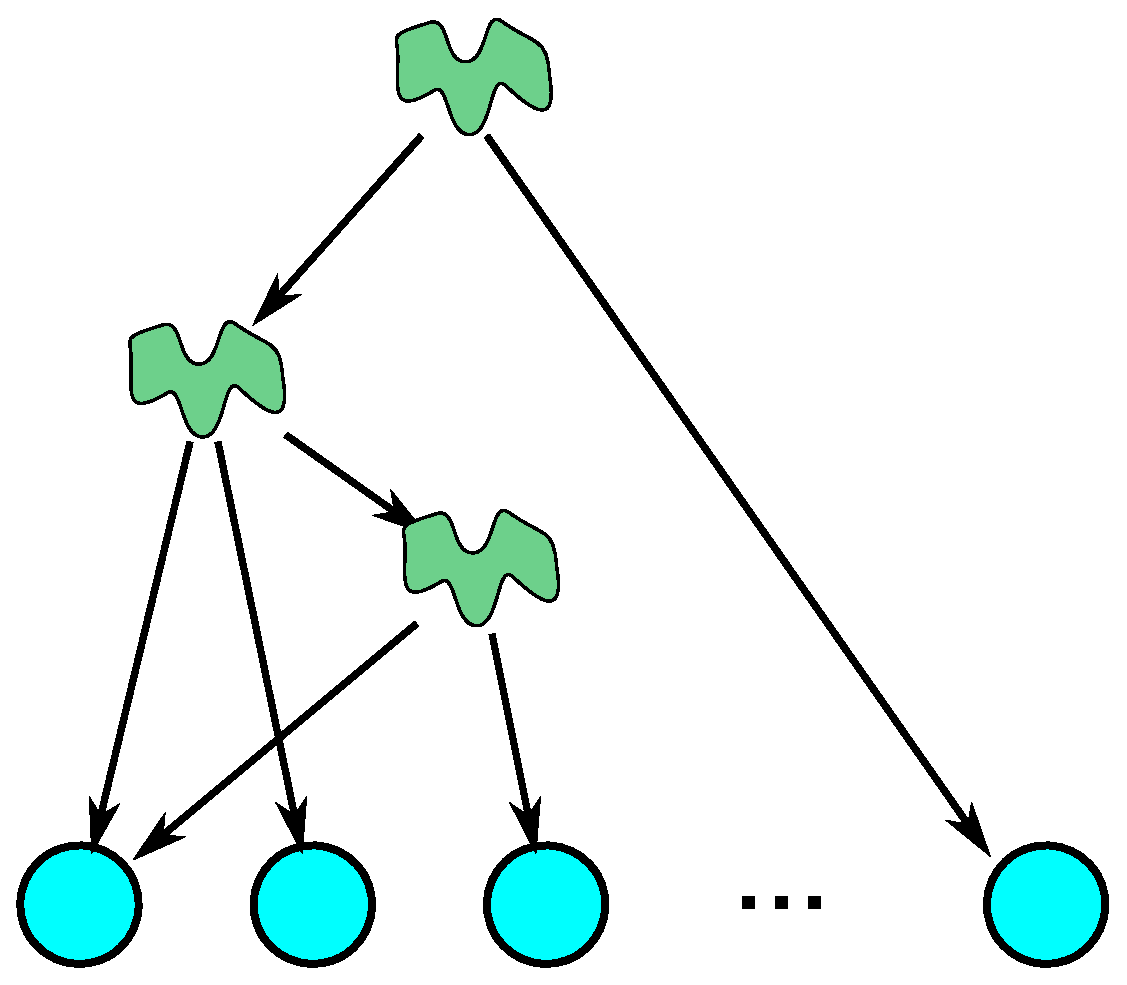
\includegraphics[width=0.5\textwidth]{\lyxdot \lyxdot /diagrams/sparseHierarchyGraph2}}\par\end{centering}


\caption{\only<1-3>{Probabilistic non-linear dimensional reduction.}\only<4>{Hierarchical
model (sparse connectivity).}\only<5>{Hierarchy of non-linear dimensional
reductions (\textbf{this talk}).} \vspace{-1cm}
}
\end{figure}


\end{block}

\lyxframeend{}\section{GP-LVM}


\lyxframeend{}\subsection{Mathematical Foundations}


\lyxframeend{}\lyxframe{Notation}

\begin{block}
{}

\begin{center}$q$--- dimension of latent/embedded space\\
$d$--- dimension of data space\\
$n$--- number of data points\par\end{center}

\begin{center}centred data, $\mathbf{Y}=\left[\mathbf{y}_{1,:},\dots,\mathbf{y}_{n,:}\right]^{\textrm{T}}=\left[\mathbf{y}_{:,1},\dots,\mathbf{y}_{:,d}\right]\in\Re^{n\times d}$\\
latent variables, $\mathbf{X}=\left[\mathbf{x}_{1,:},\dots,\mathbf{x}_{n,:}\right]^{\textrm{T}}=\left[\mathbf{x}_{:,1},\dots,\mathbf{x}_{:,q}\right]\in\Re^{n\times q}$\\
mapping matrix, $\mathbf{W}\in\Re^{d\times q}$\par\end{center}

\begin{center}$\mathbf{a}_{i,:}$ is a vector from the $i$th row
of a given matrix $\mathbf{A}$\\
$\mathbf{a}_{:,j}$ is a vector from the $j$th row of a given matrix
$\mathbf{A}$\par\end{center}

\end{block}

\lyxframeend{}\lyxframe{Reading Notation}

\begin{block}
{$\mathbf{X}$ and $\mathbf{Y}$ are \emph{design matrices}}
\begin{itemize}
\item Covariance given by $n^{-1}\mathbf{Y}^{\textrm{T}}\mathbf{Y}$.
\item Inner product matrix given by $\mathbf{Y}\mathbf{Y}^{\textrm{T}}$.
\end{itemize}
\end{block}

\lyxframeend{}\lyxframe{Linear Dimensionality Reduction}

\begin{block}
{Linear Latent Variable Model}
\begin{itemize}
\item Represent data, $\mathbf{Y}$, with a lower dimensional set of latent
variables $\mathbf{X}$.
\item Assume a linear relationship of the form\[
\mathbf{y}_{i,:}=\mathbf{W}\mathbf{x}_{i,:}+\boldsymbol{\eta}_{i,:},\]
where \[
\eta_{i,:}\sim N\left(\mathbf{0},\sigma^{2}\mathbf{I}\right).\]

\end{itemize}
\end{block}

\lyxframeend{}\lyxframe{Linear Latent Variable Model I}

\begin{centercolumns}%{}


\column{5cm}

\begin{block}
{Dual Probabilistic PCA}
\begin{itemize}
\item <1->Define \emph{linear-Gaussian relationship} between latent variables
and data.
\item <2->\textbf{Novel} Latent variable approach:

\begin{itemize}
\item <3->Define Gaussian prior over \emph{parameters}, $\mathbf{W}$.
\item <4->Integrate out \emph{parameters}.
\end{itemize}
\end{itemize}
\end{block}

\column{5cm}

\begin{block}
{}

\begin{center}\includegraphics<1-4>[width=0.5\textwidth]{../../../gplvm/tex/diagrams/gplvmGraph}\par\end{center}

\vspace{-1cm}


\begin{center}{\scriptsize \only<1-4>{\[
p\left(\mathbf{Y}|\mathbf{X},\mathbf{W}\right)=\prod_{i=1}^{n}N\left(\mathbf{y}_{i,:}|\mathbf{W}\mathbf{x}_{i,:},\sigma^{2}\mathbf{I}\right)\]
}\only<3-4>{\[
p\left(\mathbf{W}\right)=\prod_{i=1}^{d}N\left(\mathbf{w}_{i,:}|\mathbf{0},\mathbf{I}\right)\]
}\only<4->{\[
p\left(\mathbf{Y}|\mathbf{X}\right)=\prod_{j=1}^{d}N\left(\mathbf{y}_{:,j}|\mathbf{0},\mathbf{X}\mathbf{X}^{\mbox{T}}+\sigma^{2}\mathbf{I}\right)\]
}}\par\end{center}{\scriptsize \par}

\end{block}
\end{centercolumns}%{}

\lyxframeend{}\lyxframe{Linear Latent Variable Model II}

\begin{block}
{\only<1-2>{Dual} Probabilistic PCA Max. Likelihood Soln {\scriptsize \only<1-2>{\citep{Lawrence:gplvm03,Lawrence:pnpca05}}}
{\scriptsize \only<3>{\citep{Tipping:probpca99}}}}

\begin{center}\includegraphics<1>[width=0.25\textwidth]{../../../gplvm/tex/diagrams/gplvmGraph}\par\end{center}

\begin{center}{\scriptsize \vspace{-1cm}
\only<1>{\[
p\left(\mathbf{Y}|\mathbf{X}\right)=\prod_{j=1}^{d}N\left(\mathbf{y}_{:,j}|\mathbf{0},\mathbf{X}\mathbf{X}^{\mbox{T}}+\sigma^{2}\mathbf{I}\right)\]
}\only<2>{\[
p\left(\mathbf{Y}|\mathbf{X}\right)=\prod_{j=1}^{d}N\left(\mathbf{y}_{:,j}|\mathbf{0},\mathbf{K}\right),\,\,\,\,\,\,\,\mathbf{K}=\mathbf{X}\mathbf{\mathbf{X}}^{\mbox{T}}+\sigma^{2}\mathbf{I}\]
\[
\log p\left(\mathbf{Y}|\mathbf{X}\right)=-\frac{d}{2}\log\left|\mathbf{K}\right|-\frac{1}{2}\mbox{tr}\left(\mathbf{K}^{-1}\mathbf{Y}\mathbf{Y}^{\mbox{T}}\right)+\mbox{const.}\]
If $\mathbf{U}_{q}^{\prime}$ are first $q$ principal eigenvectors
of $d^{-1}\mathbf{Y}\mathbf{Y}^{\mbox{T}}$ and the corresponding
eigenvalues are $\Lambda_{q}$,\[
\mathbf{X}=\mathbf{U^{\prime}}_{q}\mathbf{L}\mathbf{V}^{\mbox{T}},\,\,\,\,\,\,\,\mathbf{L}=\left(\Lambda_{q}-\sigma^{2}\mathbf{I}\right)^{\frac{1}{2}}\]
where $\mathbf{V}$ is an arbitrary rotation matrix. }\only<3>{\[
p\left(\mathbf{Y}|\mathbf{W}\right)=\prod_{i=1}^{n}N\left(\mathbf{y}_{i,:}|\mathbf{0},\mathbf{C}\right),\,\,\,\,\,\,\,\mathbf{C}=\mathbf{W}\mathbf{W}^{\mbox{T}}+\sigma^{2}\mathbf{I}\]
\[
\log p\left(\mathbf{Y}|\mathbf{W}\right)=-\frac{n}{2}\log\left|\mathbf{C}\right|-\frac{1}{2}\mbox{tr}\left(\mathbf{C}^{-1}\mathbf{Y}^{\mbox{T}}\mathbf{Y}\right)+\mbox{const.}\]
If $\mathbf{U}_{q}$ are first $q$ principal eigenvectors of $n^{-1}\mathbf{Y}^{\mbox{T}}\mathbf{Y}$
and the corresponding eigenvalues are $\Lambda_{q}$,\[
\mathbf{W}=\mathbf{U}_{q}\mathbf{L}\mathbf{V}^{\mbox{T}},\,\,\,\,\,\,\,\mathbf{L}=\left(\Lambda_{q}-\sigma^{2}\mathbf{I}\right)^{\frac{1}{2}}\]
where $\mathbf{V}$ is an arbitrary rotation matrix. }}\par\end{center}{\scriptsize \par}

\end{block}

\lyxframeend{}\lyxframe{Equivalence of Formulations}

\begin{block}
{The Eigenvalue Problems are equivalent}
\begin{itemize}
\item Solution for Probabilistic PCA (solves for the mapping)


{\footnotesize \[
\mathbf{Y}^{\mbox{T}}\mathbf{Y}\mathbf{U}_{q}=\mathbf{U}_{q}\Lambda_{q}\,\,\,\,\,\,\,\,\,\,\mathbf{W}=\mathbf{U}_{q}\mathbf{L}\mathbf{V}^{\mbox{T}}\]
}{\footnotesize \par}

\item Solution for Dual Probabilistic PCA (solves for the latent positions)


{\footnotesize \[
\mathbf{Y}\mathbf{Y}^{\mbox{T}}\mathbf{U}_{q}^{\prime}=\mathbf{U}_{q}^{\prime}\Lambda_{q}\,\,\,\,\,\,\,\,\,\,\mathbf{X}=\mathbf{U}_{q}^{\prime}\mathbf{L}\mathbf{V}^{\mbox{T}}\]
}{\footnotesize \par}

\item Equivalence is from{\footnotesize \[
\mathbf{U}_{q}=\mathbf{Y}^{\mbox{T}}\mathbf{U}_{q}^{\prime}\Lambda_{q}^{-\frac{1}{2}}\]
}{\footnotesize \par}
\end{itemize}
\end{block}

\lyxframeend{}\lyxframe{Non-Linear Latent Variable Model}

\begin{centercolumns}%{}


\column{5cm}

\begin{block}
{Dual Probabilistic PCA}

\only<1>{

\begin{itemize}
\item Define \emph{linear-Gaussian relationship} between latent variables
and data.
\item \textbf{Novel} Latent variable approach:

\begin{itemize}
\item Define Gaussian prior over \emph{parameteters}, $\mathbf{W}$.
\item Integrate out \emph{parameters}.
\end{itemize}
\end{itemize}
}\only<2->{

\begin{itemize}
\item <2->Inspection of the marginal likelihood shows ...

\begin{itemize}
\item <3->The covariance matrix is a covariance function.
\item <4->We recognise it as the `linear kernel'.
\item <5->We call this the Gaussian Process Latent Variable model (GP-LVM).
\end{itemize}
\end{itemize}
}

\end{block}

\column{5cm}

\begin{block}
{}

\begin{center}\includegraphics<1->[width=0.5\textwidth]{../../../gplvm/tex/diagrams/gplvmGraph}\par\end{center}

\vspace{-1cm}


\begin{center}{\scriptsize \only<1>{\[
p\left(\mathbf{Y}|\mathbf{X},\mathbf{W}\right)=\prod_{i=1}^{n}N\left(\mathbf{y}_{i,:}|\mathbf{W}\mathbf{x}_{i,:},\sigma^{2}\mathbf{I}\right)\]
\[
p\left(\mathbf{W}\right)=\prod_{i=1}^{d}N\left(\mathbf{w}_{i,:}|\mathbf{0},\mathbf{I}\right)\]
}\only<1-2>{\[
p\left(\mathbf{Y}|\mathbf{X}\right)=\prod_{j=1}^{d}N\left(\mathbf{y}_{:,j}|\mathbf{0},\mathbf{X}\mathbf{X}^{\mbox{T}}+\sigma^{2}\mathbf{I}\right)\]
}\only<3->{\[
p\left(\mathbf{Y}|\mathbf{X}\right)=\prod_{j=1}^{d}N\left(\mathbf{y}_{:,j}|\mathbf{0},\mathbf{K}\right)\]
}\only<3-4>{\[
\mathbf{K}=\mathbf{X}\mathbf{X}^{\mbox{T}}+\sigma^{2}\mathbf{I}\]
}\only<4>{This is a product of Gaussian processes with linear kernels.}\only<5>{\[
\mathbf{K}=?\]
Replace linear kernel with non-linear kernel for non-linear model.}}\par\end{center}{\scriptsize \par}

\end{block}
\end{centercolumns}%{}

\lyxframeend{}\lyxframe{Stick Man}

\begin{block}
{Generalization with less Data than Dimensions}
\begin{itemize}
\item Powerful uncertainty handling of GPs leads to suprising properties.
\item Non-linear models can be used where there are fewer data points than
dimensions \emph{without overfitting}.
\item Example: Modelling a stick man in 102 dimensions with 55 data points!
\end{itemize}
\end{block}

\lyxframeend{}\lyxframe{Stick Man II}

\begin{block}
{\texttt{demStick1}}

%
\begin{figure}
\begin{centering}\only<1>{\vspace{4cm}
}\only<2>{\includegraphics[width=0.5\textwidth]{\lyxdot \lyxdot /\lyxdot \lyxdot /\lyxdot \lyxdot /fgplvm/tex/diagrams/demStick1Connected}}\par\end{centering}


\caption{The latent space for the stick man motion capture data. \vspace{-1cm}
}
\end{figure}


\end{block}

\lyxframeend{}\subsection{Dynamics}


\lyxframeend{}\lyxframe{Adding Dynamics}

\begin{block}
{MAP Solutions for Dynamics Models}
\begin{itemize}
\item Introduce dynamical model in latent space.

\begin{itemize}
\item Marginalising such dynamics is intractable.
\item But: \textbf{MAP solutions} are trivial to implement.
\end{itemize}
\item \citet{Wang:gpdm05} suggest using a auto regressive Gaussian Process.
\item Here we use a regressive Gaussian process.


$p\left(\mathbf{Y}|\mathbf{t}\right)=\int p\left(\mathbf{Y}|\mathbf{X}\right)p\left(\mathbf{X}|\mathbf{t}\right)d\mathbf{X}$

\end{itemize}
\end{block}

\lyxframeend{}\lyxframe{Regressive Dynamics}

\begin{block}
{Direct use of Time Variable}
\begin{itemize}
\item Take $\mathbf{t}$ as an input, use a prior $p\left(\mathbf{X}|\mathbf{t}\right)$.
\item User a Gaussian process prior for $p\left(\mathbf{X}|\mathbf{t}\right).$
\item Also allows us to consider variable sample rate data.
\end{itemize}
\end{block}

\lyxframeend{}\lyxframe{Motion Capture Results}

\begin{block}
{\texttt{demStick1} and \texttt{demStick5}}

%
\begin{figure}
\begin{centering}\only<1>{\vspace{3cm}
}\only<2>{\includegraphics[width=0.45\textwidth]{\lyxdot \lyxdot /\lyxdot \lyxdot /\lyxdot \lyxdot /fgplvm/tex/diagrams/demStick1Connected}\includegraphics[width=0.45\textwidth]{\lyxdot \lyxdot /\lyxdot \lyxdot /\lyxdot \lyxdot /fgplvm/tex/diagrams/demStick5Connected}}\par\end{centering}


\caption{The latent space for the motion capture data without dynamics (\emph{left})
and with regressive dynamics (\emph{right}) based on an RBF kernel. }
\end{figure}


\end{block}

\lyxframeend{}\section{Hierarchical GP-LVM}


\lyxframeend{}\lyxframe{Hierarchical GP-LVM}

\begin{block}
{Stacking Gaussian Processes}
\begin{itemize}
\item Regressive dynamics provides a \emph{simple hierarchy}.

\begin{itemize}
\item The input space of the GP is governed by another GP.
\end{itemize}
\item By stacking GPs we can consider more complex hierarchies.
\end{itemize}
\end{block}

\lyxframeend{}\lyxframe{Hierarchical GP-LVM}

\begin{block}
{Stacking GP-LVMs}

%
\begin{figure}
\begin{centering}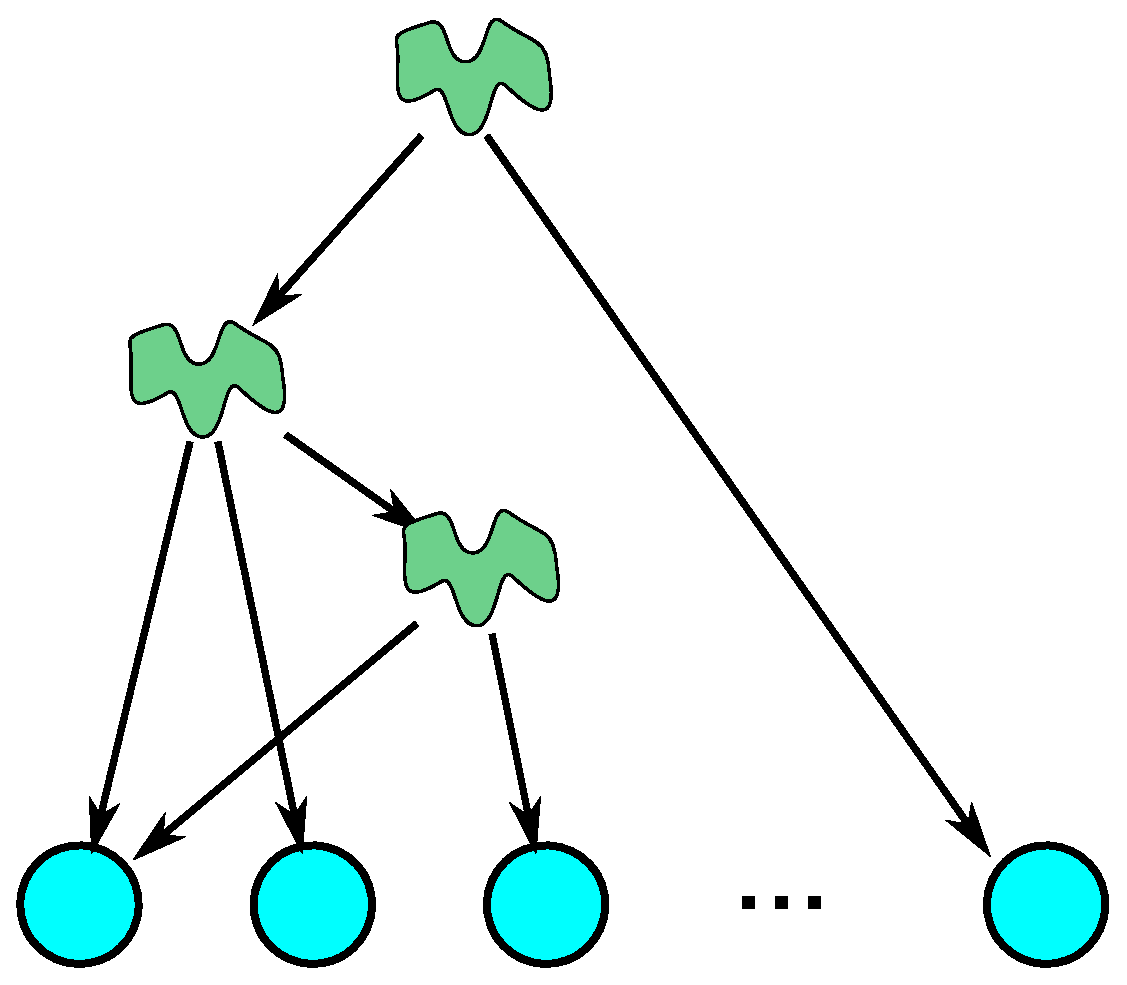
\includegraphics[width=0.25\textwidth]{\lyxdot \lyxdot /diagrams/sparseHierarchyGraph2}\par\end{centering}
\end{figure}


\begin{itemize}
\item This provides a route to incoporate conditional independencies.
\item Ideally we should marginalise latent spaces

\begin{itemize}
\item In practice we seek \textbf{MAP solutions}.
\end{itemize}
\end{itemize}
\end{block}

\lyxframeend{}\subsection{Two Correlated Subjects}


\lyxframeend{}\lyxframe{Two Correlated Subjects}

\begin{centercolumns}%{}


\column{5cm}

\begin{block}
{}
\begin{itemize}
\item Simple hieararchy:

\begin{itemize}
\item Motion capture data with two subjects.
\end{itemize}
\item Subjects interact: approach each other and `high five'.
\item Model as a very simple tree.
\end{itemize}
\end{block}

\column{5cm}

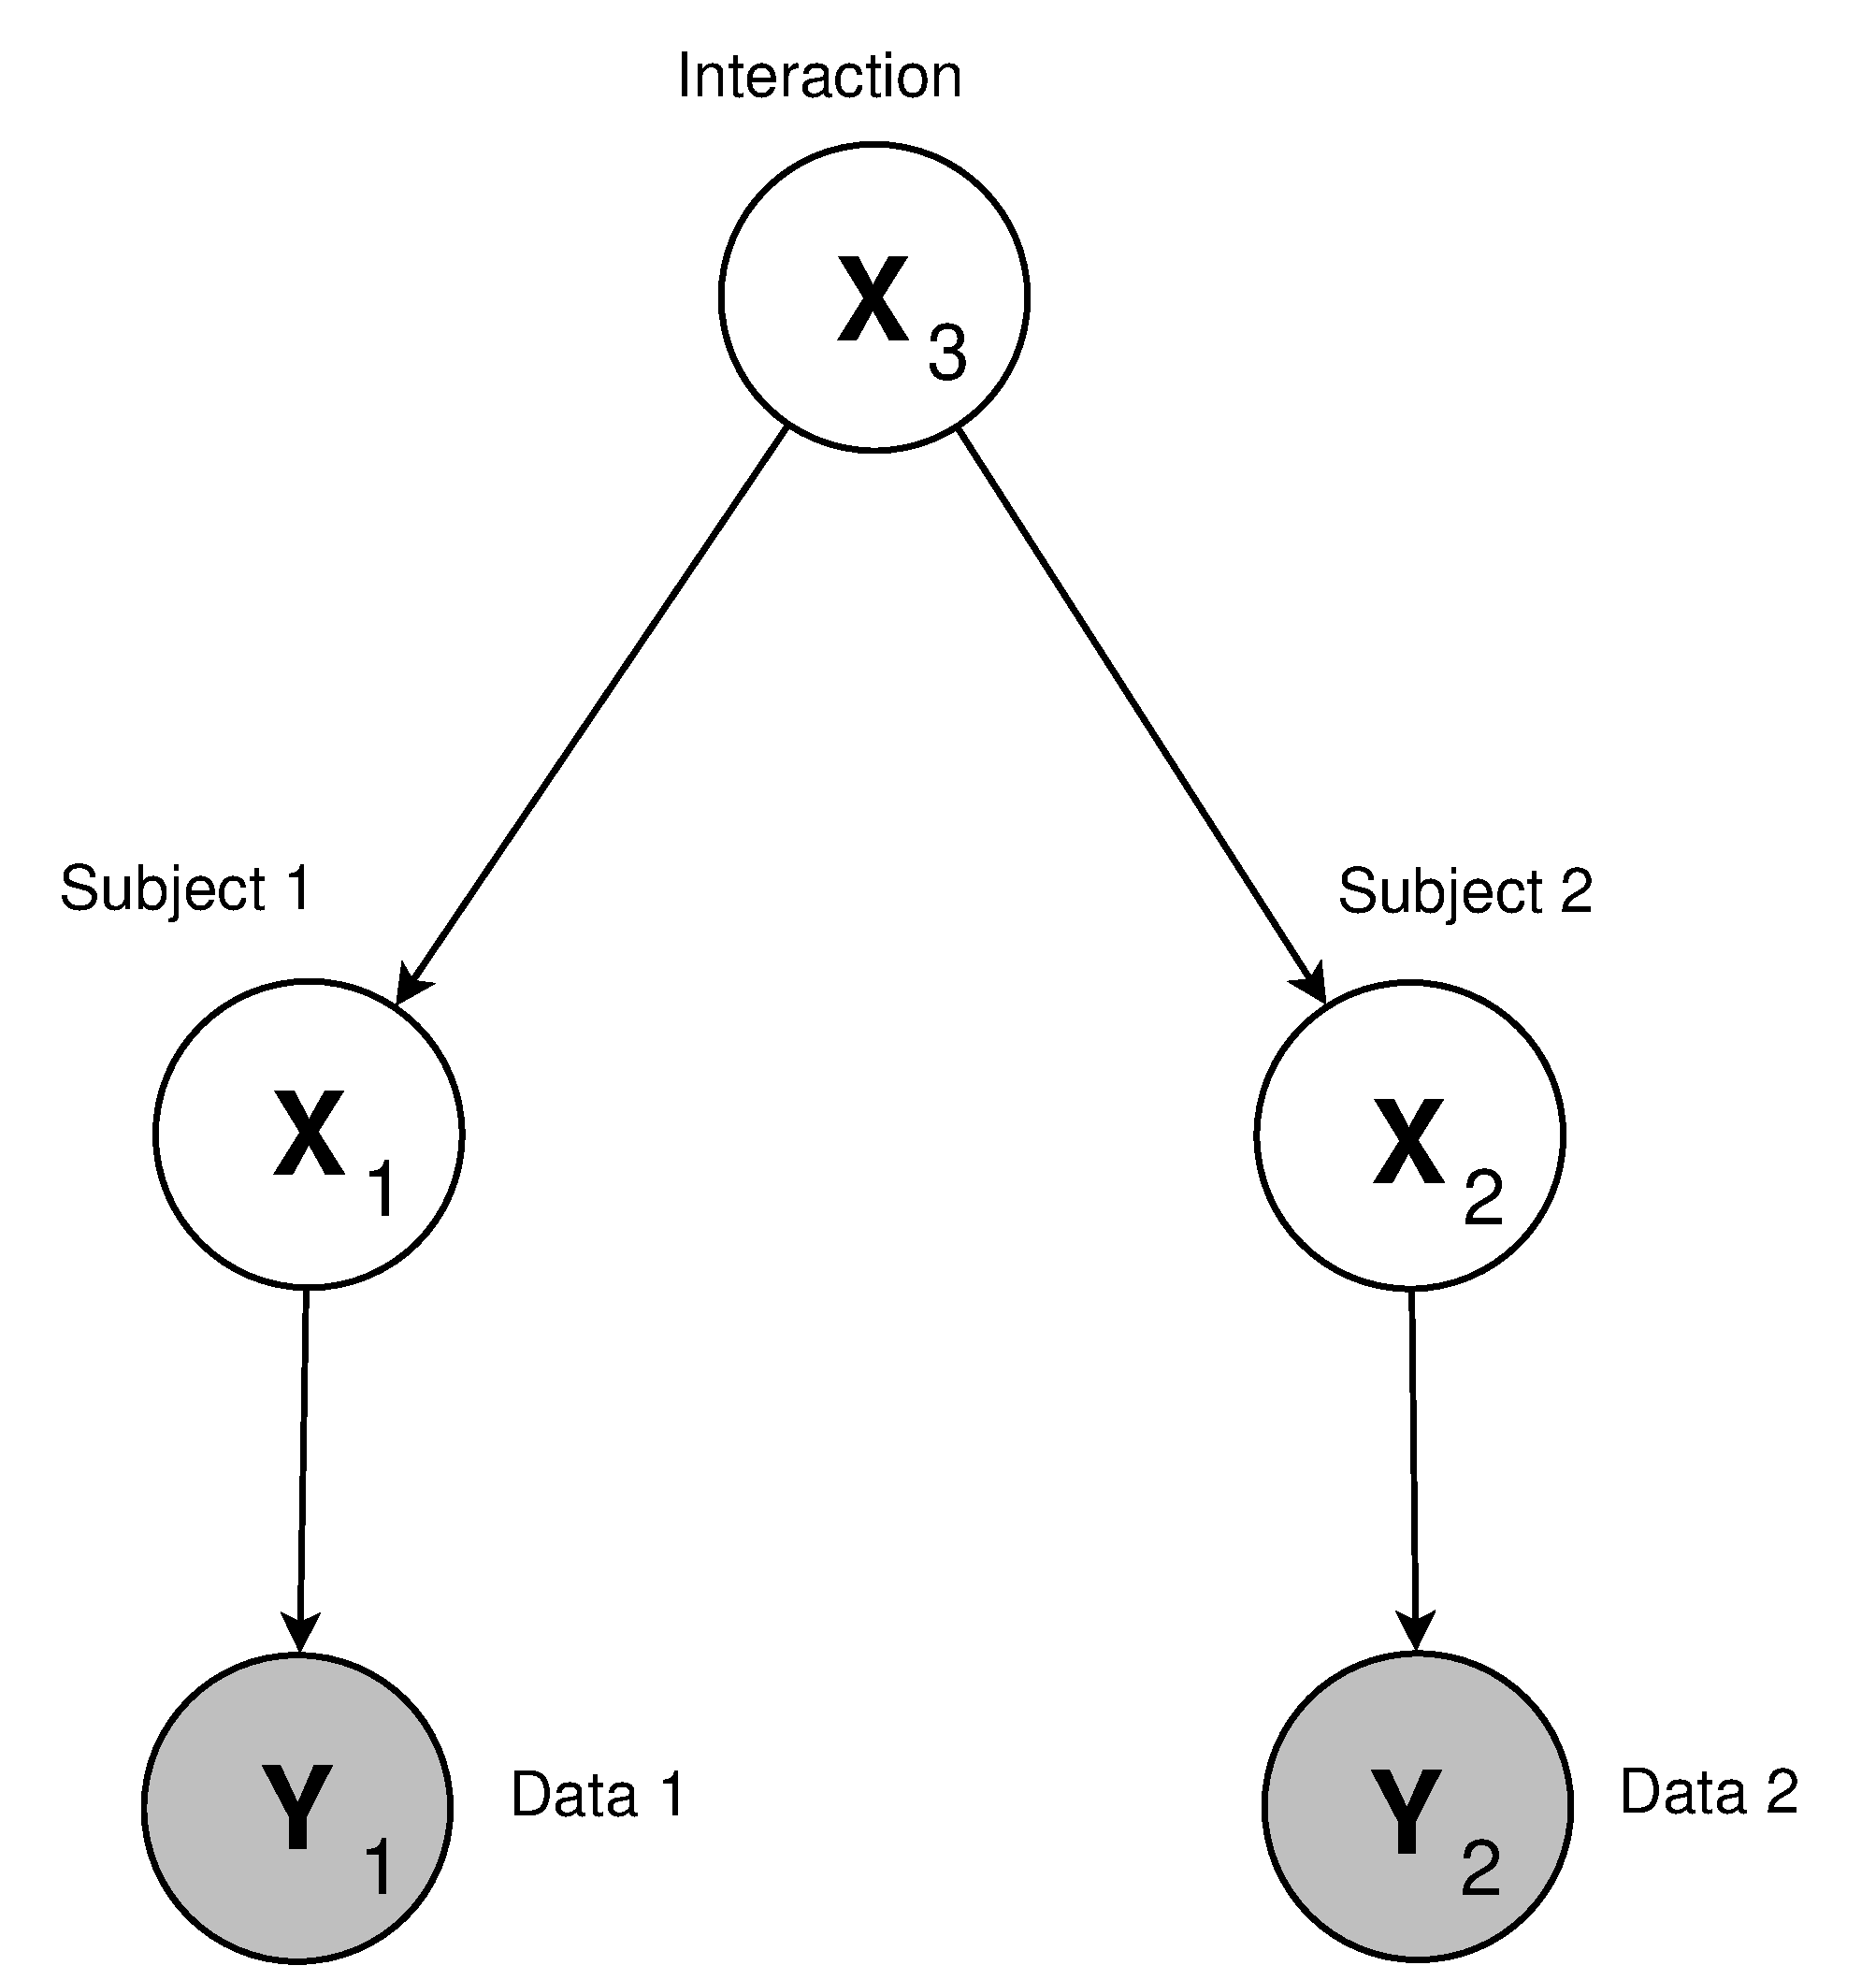
\includegraphics[width=0.7\columnwidth]{\lyxdot \lyxdot /diagrams/twoSubjects}

\end{centercolumns}%{}
\begin{block}
{\footnotesize {}}{\footnotesize \par}

{\footnotesize $p\left(\mathbf{Y}_{1},\mathbf{Y}_{2}\right)=\int p\left(\mathbf{Y}_{1}|\mathbf{X}_{1}\right)\int p\left(\mathbf{Y}_{2}|\mathbf{X}_{2}\right)\int p\left(\mathbf{X}_{1}|\mathbf{X}_{3}\right)p\left(\mathbf{X}_{2}|\mathbf{X}_{3}\right)d\mathbf{X}_{1}d\mathbf{X}_{2}d\mathbf{X}_{3}$}{\footnotesize \par}

\end{block}

\lyxframeend{}\lyxframe{Two Correlated Subjects}

\begin{block}
{\texttt{demHighFive1}}

%
\begin{figure}
\begin{centering}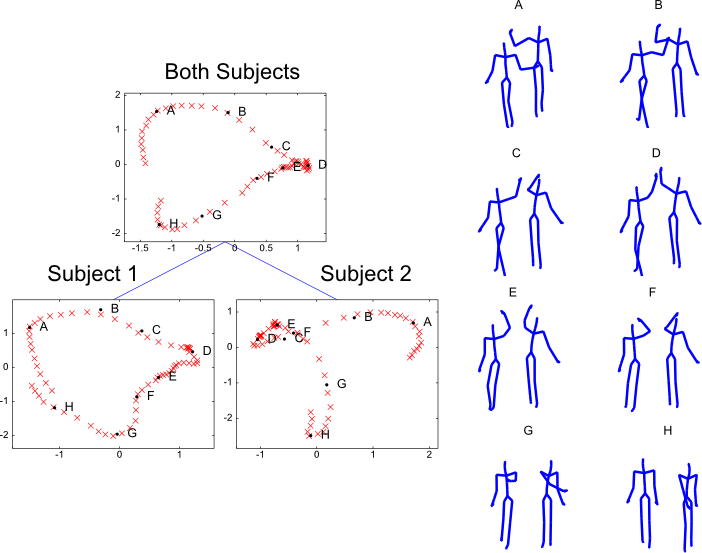
\includegraphics[width=0.8\textheight]{C:/cygwin/home/neil/mlprojects/hgplvm/tex/diagrams/demHighFive_talk}\par\end{centering}


\caption{Hierarchical model of a 'high five'.}
\end{figure}


\end{block}

\lyxframeend{}\subsection{Subject Decomposition}


\lyxframeend{}\lyxframe{Within Subject Hierarchy}

\begin{block}
{Decomposition of Body}

%
\begin{figure}
\begin{centering}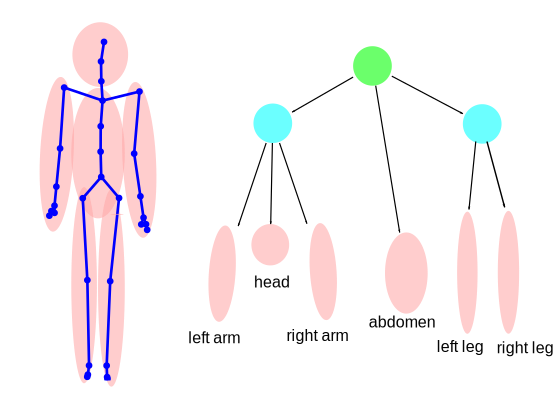
\includegraphics[width=0.7\textheight]{C:/cygwin/home/neil/mlprojects/hgplvm/tex/diagrams/stickHierarchy}\par\end{centering}


\caption{Decomposition of a subject.}
\end{figure}


\end{block}

\lyxframeend{}\lyxframe{Single Subject Run/Walk}

\begin{block}
{\texttt{demRunWalk1}}

%
\begin{figure}
\begin{centering}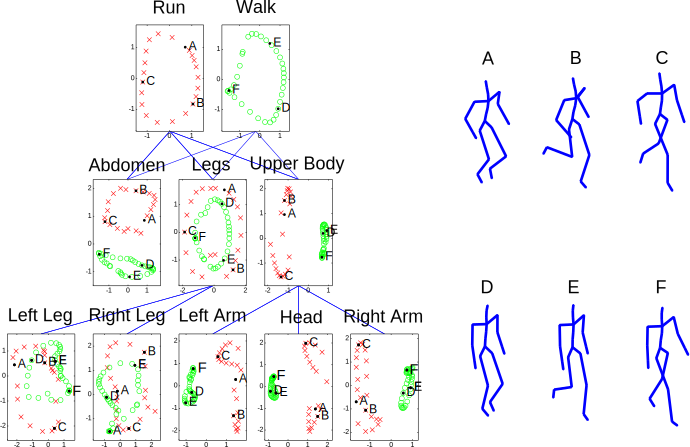
\includegraphics[width=0.8\textheight]{C:/cygwin/home/neil/mlprojects/hgplvm/tex/diagrams/demWalkRun_talk}\par\end{centering}


\caption{Hierarchical model of a walk and a run.}
\end{figure}


\end{block}

\lyxframeend{}\section{Discussion}


\lyxframeend{}\subsection{Overfitting}


\lyxframeend{}\lyxframe{Overfitting}

\begin{block}
{More parameters than data}
\begin{itemize}
\item Large number of parameters: why doesn't it overfit?
\item Standard GP-LVM: parameters increase linearly $\frac{q}{d}\times N$,
$q<d$ .
\item HGP-LVM: adding more latent variables (parameters), will we overfit? 

\begin{itemize}
\item Upper levels only regularise the leaf nodes: if the leaf nodes don't
overfit model won't.
\item Best likelihood obtained by \emph{removing regularisation}. \emph{}
\item Counter this potential problem in two ways. 

\begin{enumerate}
\item Provide a fixed dynamical prior at the top level. 
\item Constraine the noise variance of each non-leaf Gaussian process to
$1\times10^{-6}$.
\end{enumerate}
\end{itemize}
\end{itemize}
\end{block}

\lyxframeend{}\subsection{Summary}


\lyxframeend{}\lyxframe{Summary}

\begin{block}
{Conclusions}
\begin{itemize}
\item GP-LVM is a Probabilistic Non-Linear Generalisation of PCA.
\item We can stack GP-LVMs to provide:

\begin{itemize}
\item A dynamical model.
\item A hierarchical decomposition of our data.
\end{itemize}
\item MAP Solutions still provide interesting decompositions.
\end{itemize}
\end{block}
\appendix

\lyxframeend{}\lyxframe{References}

{\tiny \bibliographystyle{abbrvnat}
\bibliography{lawrence,other,zbooks}
}{\tiny \par}


\lyxframeend{}


\end{document}
